\documentclass[11pt]{article}

\usepackage[margin=1in]{geometry}
\usepackage[T1]{fontenc}
\usepackage[utf8]{inputenc}
\usepackage{lmodern}
\usepackage{microtype}
\usepackage{amsmath,amssymb,amsthm,mathtools}
\usepackage{booktabs}
\usepackage{longtable}
\usepackage{tabularx}
\usepackage{array}
\usepackage{enumitem}
\usepackage{xcolor}
\usepackage{hyperref}
\usepackage{xurl}
\usepackage{tikz}
\usetikzlibrary{arrows.meta,positioning,fit,calc,shapes.geometric,shapes.multipart}

\hypersetup{
  colorlinks=true,
  linkcolor=blue!50!black,
  urlcolor=blue!50!black,
  citecolor=blue!50!black,
  pdftitle={Aft Fault Tolerance Yellow Paper},
  pdfauthor={IOI}
}

\newtheorem{theorem}{Theorem}
\newtheorem{proposition}{Proposition}

\newcommand{\AFT}{\textsc{AFT}}
\newcommand{\code}[1]{\texttt{#1}}
\newcommand{\term}[1]{\textit{#1}}
\newcommand{\suchthat}{\;|\;}

\setlength{\emergencystretch}{3em}

\title{Aft Fault Tolerance: Relay-Free Deterministic 99\% Byzantine Tolerance in Pure Software}
\author{IOI}
\date{March 17, 2026}

\begin{document}

\maketitle

\begin{abstract}
\AFT{} is a family of consensus and settlement constructions for
high-throughput ordering, guardian-backed base finality, proof-carrying
canonical ordering, and deterministic release of irreversible effects. Its
central move is to stop treating dense positive voting as the only possible
source of ordering truth. Instead, \AFT{} separates throughput-critical
publication and chain progression from authority-critical proof verification,
omission detection, and effect collapse.

The protocol family has four interacting surfaces. \term{GuardianMajority}
supplies the production base-finality path: a validator quorum certificate is
necessary but not sufficient, because each proposal must also carry a
registered guardian committee certificate anchored into shared evidence.
\term{CanonicalOrdering} supplies the proof-carrying ordering path: a slot
order is accepted because a canonical certificate is uniquely valid and
recoverable from public inputs, not because a dense validator quorum voted the
order into existence. \term{Asymptote} supplies the sealing path for
irreversible effects: \code{BaseFinal} chain progress is upgraded to
\code{SealedFinal} through deterministic witness or observer-backed collapse,
with canonical observer challenges dominating unsafe releases.
\term{NestedGuardian} supplies a
witness-augmented research path for layered threshold constructions.

This paper is self-contained and normative for the protocol family. Its
ordering subtheorem remains \code{99\%} equal-authority ordering consensus
under explicit bulletin-publication, cutoff, omission, extractability, and
proof-soundness assumptions. The stronger repository-level claim is
\code{relay-free, coordinator-free, pure-software deterministic 99\%
Byzantine Tolerance}: for each closed slot boundary there exists at most one
admissible public execution object, every conflicting fully specified
candidate admits a short public contradiction witness, durable state advances
only through canonical collapse, and sealed-effect release is bound to the
same collapse surface. This is not a claim of unconditional classical
\code{99\% Byzantine agreement} in the ordinary dense-vote permissioned model.
Unlike classical partially synchronous Byzantine agreement, which requires
\(> 2/3\) honest participation to guarantee progress under worst-case
asynchrony, \AFT{} derives safety without trusted relays, privileged
coordinators, TEEs, or dense positive quorum intersection. Safety comes from
proof-carrying public evidence, dominant negative proofs, deterministic public
extraction, and collapse-gated durability; accountable publication and
validator removal remain operational reinforcement, not the source of
correctness.
\end{abstract}

\section{Scope and Status}

This paper contains the full architectural and theorem-level description of
the current \AFT{} family. It does not require any companion prose
specification to be understood.

The repository currently instantiates the following protocol surfaces:

\begin{itemize}[leftmargin=1.5em]
\item \code{GuardianMajority} as the production guardian-backed base-finality
mode.
\item \code{Asymptote} as the two-tier sealing and irreversible-effects mode.
\item \code{CanonicalOrdering} through the live
\code{CommittedSurfaceV1} certificate path attached to \code{Asymptote}
blocks.
\item \code{NestedGuardian} as an experimental witness-augmented mode with
safety proofs and bounded operational checks, but not a finished composed
liveness theorem.
\end{itemize}

Implementation correspondence is included below as exact symbol references.
That section is non-normative. The protocol and theorem content of the paper
stands on its own.

The strongest theorem surface of the live runtime is now the
public-state-continuity claim: \AFT{} claims not only \code{99\%}
equal-authority ordering for the ordering layer, but relay-free,
coordinator-free, pure-software deterministic \code{99\% Byzantine Tolerance}
for durable ordering and sealed-effect safety over the explicit
public-state-continuity substrate.

\section{Problem Statement}

Classical permissioned Byzantine fault tolerance ties deterministic safety to
dense positive voting by a large honest majority. Under that model, honest
inclusion, total-order agreement, and finality all depend on most validators
remaining both correct and available. That is the right model when the
protocol is allowed to pay dense coordination cost and accept classical
\(3f+1\)-style thresholds. It is the wrong model for a system that wants all
of the following simultaneously:

\begin{itemize}[leftmargin=1.5em]
\item high-throughput publication and chain progression,
\item equal-authority participation at the validator layer,
\item deterministic rejection of incomplete or conflicting ordered views,
\item stronger accountability than ``someone must have voted wrong,''
\item deterministic gating of irreversible effects.
\end{itemize}

\AFT{} therefore changes the object of agreement.

Instead of asking:

\begin{itemize}[leftmargin=1.5em]
\item ``Which order did the validator quorum choose?''
\end{itemize}

it asks:

\begin{itemize}[leftmargin=1.5em]
\item ``Which order certificate is uniquely valid for this slot, and which
effects are admissible after deterministic collapse?''
\end{itemize}

The family-level design goals are:

\begin{itemize}[leftmargin=1.5em]
\item keep ordering and publication sparse on the hot path,
\item keep effect release fail-closed,
\item make omissions and conflicts objectively provable,
\item keep all validators equally eligible to reveal the canonical order,
\item move authority from dense yes-votes to verifiable evidence.
\end{itemize}

\section{Thought Experiment: The Port of Public Manifests and Release Seals}

Imagine an international port that handles ordinary cargo and hazardous cargo.

Every ship that wants to unload during tide \(h\) must post its cargo manifest
to a public harbor board before the closing bell \(\tau_h\). The bell is not a
private clock in the harbor master's office. It is a certified public event.
Once the bell rings, the harbor office takes every admissible manifest,
applies the published tide lottery \(R_h\), and derives one canonical docking
docket \(O_h\).

The office does not ask every captain to vote on the exact order of every
container. It asks a simpler question: has someone produced the one valid
docket certificate for the manifests that were publicly posted before the bell?
If any dockworker can prove that an admissible manifest was omitted from the
announced docket, that docket is rejected immediately.

Ordinary unloading may begin once the berth assignment is base-final.
Hazardous cargo is stricter. It may leave the port only after one of two
things happens:

\begin{itemize}[leftmargin=1.5em]
\item the required independent inspector guilds each sign a release
certificate, or
\item a deterministically assigned set of external captains publishes a public
inspection transcript surface, the public red-flag board remains empty through
the close bell, and the port issues the unique release docket implied by that
surface.
\end{itemize}

Any valid red flag aborts release. The cargo does not ``probably'' leave the
port. It does not leave.

Most of the port can be chaotic. Captains can lie, stall, or collude. What
they cannot do is create a second valid docket for the same tide or a second
valid hazardous-cargo release order, provided the public manifest board
remains recoverable and the decisive proof surface stays objectively
checkable.

\begin{figure}[t]
\centering
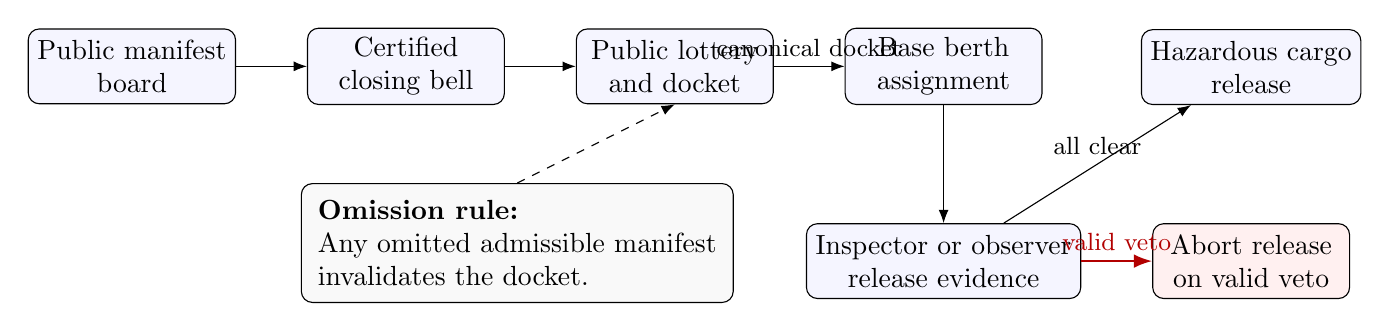
\begin{tikzpicture}[
  node distance=1.35cm and 0.9cm,
  >=Latex,
  block/.style={draw, rounded corners, align=center, minimum width=2.5cm, minimum height=0.95cm, fill=blue!4},
  abort/.style={draw, rounded corners, align=center, minimum width=2.5cm, minimum height=0.95cm, fill=red!6},
  labelbox/.style={draw, rounded corners, align=left, inner sep=6pt, fill=gray!5}
]
\node[block] (board) {Public manifest\\board};
\node[block, right=of board] (cutoff) {Certified\\closing bell};
\node[block, right=of cutoff] (lottery) {Public lottery\\and docket};
\node[block, right=of lottery] (base) {Base berth\\assignment};
\node[block, below=1.5cm of base] (sealed) {Inspector or observer\\release evidence};
\node[abort, right=of sealed] (abort) {Abort release\\on valid veto};
\node[block, above=1.5cm of abort] (release) {Hazardous cargo\\release};

\draw[->] (board) -- (cutoff);
\draw[->] (cutoff) -- (lottery);
\draw[->] (lottery) -- node[above, font=\small] {canonical docket} (base);
\draw[->] (base) -- (sealed);
\draw[->] (sealed) -- node[above, font=\small] {all clear} (release);
\draw[->, thick, red!70!black] (sealed) -- node[above, font=\small] {valid veto} (abort);

\node[labelbox, below=1.0cm of lottery, xshift=-2.0cm] (omit) {
\textbf{Omission rule:}\\
Any omitted admissible manifest\\
invalidates the docket.
};
\draw[->, dashed] (omit.north) -- (lottery.south);
\end{tikzpicture}
\caption{The thought experiment behind \AFT{}: public admission, canonical
ordering, base progress, and fail-closed release.}
\end{figure}

The correspondence is direct:

\begin{center}
\small
\begin{tabularx}{\textwidth}{>{\raggedright\arraybackslash}p{0.38\textwidth} X}
\toprule
\textbf{Port object} & \textbf{\AFT{} object} \\
\midrule
Public manifest board & Bulletin / DA surface \(B_h\) \\
Certified closing bell & Canonical cutoff \(\tau_h\) \\
Tide lottery & Public randomness beacon \(R_h\) \\
Docking docket & Canonical order \(O_h\) \\
Docket certificate & Canonical-order certificate \(OCert_h\) \\
Omitted manifest challenge & Omission proof \(\Omega(h, tx)\) \\
Base berth assignment & \code{BaseFinal} \\
Independent inspector guilds & Witness committees \\
Sampled external captains & Equal-authority observers \\
Red-flag report & Canonical observer challenge \\
Hazardous cargo release seal & \code{SealObject} under \code{SealedFinal} \\
\bottomrule
\end{tabularx}
\end{center}

This thought experiment captures the essential \AFT{} move: sparse operational
progress, dense cheap verification, objective omission, and deterministic
collapse for irreversible consequences.

\section{Protocol Family Overview}

\AFT{} is best understood as four planes that compose:

\begin{center}
\small
\begin{tabularx}{\textwidth}{>{\raggedright\arraybackslash}p{0.20\textwidth} >{\raggedright\arraybackslash}p{0.22\textwidth} >{\raggedright\arraybackslash}p{0.24\textwidth} X}
\toprule
\textbf{Plane} & \textbf{Purpose} & \textbf{Throughput-critical work} & \textbf{Authority object} \\
\midrule
Dissemination / bulletin plane & Publish the candidate transaction surface & Data dissemination and bulletin commitments & Public bulletin commitment \\
Base-finality plane & Advance the chain and commit block identity & Proposal, QC formation, guardianized certification & Validator QC + guardian certificate \\
Canonical-ordering plane & Prove the unique slot order & Succinct verification, omission dominance & \(OCert_h\) \\
Sealed-effect plane & Gate irreversible effects & Asynchronous witness / observer evidence collection & \code{SealedFinalityProof} and \code{SealObject} \\
\bottomrule
\end{tabularx}
\end{center}

The protocol modes are:

\begin{center}
\small
\begin{tabularx}{\textwidth}{>{\raggedright\arraybackslash}p{0.22\textwidth} >{\raggedright\arraybackslash}p{0.48\textwidth} X}
\toprule
\textbf{Mode} & \textbf{Role} & \textbf{Current status} \\
\midrule
\code{GuardianMajority} & Production guardian-backed base finality & Production mode \\
\code{CanonicalOrdering} & Proof-carrying equal-authority ordering & Live through \code{CommittedSurfaceV1} \\
\code{Asymptote} & Two-tier sealing and sealed-effect release & Production sealing path \\
\code{NestedGuardian} & Witness-augmented layered threshold mode & Experimental / research \\
\bottomrule
\end{tabularx}
\end{center}

The key invariant is:

\[
\text{throughput-critical work} \neq \text{authority-critical work}
\]

\begin{figure}[t]
\centering
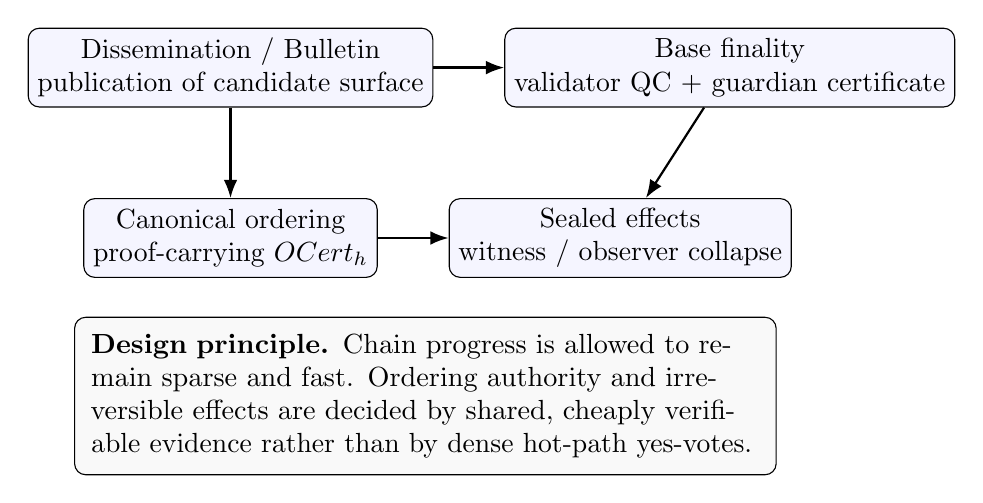
\begin{tikzpicture}[
  >=Latex,
  node distance=1.15cm and 0.9cm,
  box/.style={draw, rounded corners, align=center, minimum width=3.1cm, minimum height=1.0cm, fill=blue!4},
  note/.style={draw, rounded corners, align=left, inner sep=6pt, fill=gray!5}
]
\node[box] (bulletin) {Dissemination / Bulletin\\publication of candidate surface};
\node[box, right=of bulletin] (base) {Base finality\\validator QC + guardian certificate};
\node[box, below=of bulletin] (order) {Canonical ordering\\proof-carrying \(OCert_h\)};
\node[box, right=of order] (sealed) {Sealed effects\\witness / observer collapse};

\draw[->, thick] (bulletin) -- (base);
\draw[->, thick] (bulletin) -- (order);
\draw[->, thick] (base) -- (sealed);
\draw[->, thick] (order) -- (sealed);

\node[note, below=1.0cm of $(order)!0.5!(sealed)$, text width=0.7\textwidth] (note) {
\textbf{Design principle.}
Chain progress is allowed to remain sparse and fast.
Ordering authority and irreversible effects are decided by shared,
cheaply verifiable evidence rather than by dense hot-path yes-votes.
};
\end{tikzpicture}
\caption{\AFT{} separates publication, base progress, canonical ordering, and
sealed effect release, then recomposes them through shared evidence.}
\end{figure}

\section{System Model and Notation}
\label{sec:system-model}

\subsection{Actors}

\begin{itemize}[leftmargin=1.5em]
\item \textbf{Validator:} participates in proposal, vote, verification, and
chain execution.
\item \textbf{Guardian committee:} the registered threshold-signing committee
protecting one validator's proposal decisions.
\item \textbf{Guardian member:} an individual signer within a guardian
committee.
\item \textbf{Witness committee:} an external threshold-signing committee used
on the sealing path or in \code{NestedGuardian}.
\item \textbf{Equal-authority observer:} a validator sampled to audit a slot
under \code{Asymptote}.
\item \textbf{Registry:} the on-chain source of truth for manifests, policies,
epochs, witness sets, and verifier descriptors.
\item \textbf{Transparency log:} an append-only checkpointed evidence log for
guardian and witness statements.
\item \textbf{External verifier or gateway:} a party that checks
\code{SealObject}s and enforces replay-safe release.
\end{itemize}

\subsection{Bulletin-board time and slot model}

Consensus proceeds in heights and views. A slot is identified by
\((height, view)\). Epoch-scoped policy and committee state bind the
admissible evidence for that slot. The family should be read under a
bulletin-board recoverability model rather than a pure point-to-point timely
receipt model: safety depends on whether admissible evidence becomes publicly
retrievable by the slot cutoff, not on whether every participant receives every
message before that cutoff.

Slots are externally paced by a public cutoff object \(\tau_h\) and a public
randomness beacon \(R_h\). Honest validators that observe the same closed
public boundary derive the same ordering or sealing close-or-abort result. In
the live runtime that derivation is no longer keyed off cutoff closure alone:
the bulletin plane exports a
\term{canonical bulletin-close object} binding the bulletin commitment, the
bulletin-availability certificate, and the canonical cutoff into one public
close surface. In the current runtime slice, positive canonical-order
publication is fail-closed at this boundary: a closed-slot order certificate is
admitted only if the published bulletin entries deterministically extract the
bulletin surface bound by the canonical bulletin-close object and the carried
bulletin-availability certificate. Universal timely receipt is not required.

Let
\[
h = \text{slot height}, \quad
v = \text{slot view},
\]
\[
B_h = \text{bulletin surface admitted before cutoff }\tau_h,
\]
\[
R_h = \text{public randomness beacon for slot }h,
\]
\[
E_h = \{tx \suchthat \mathrm{Included}(tx, B_h) \wedge \mathrm{Eligible}(tx, root_{h-1})\},
\]
\[
O_h = \mathrm{CanonicalOrder}(R_h, E_h),
\]
\[
root_h = \mathrm{Execute}(root_{h-1}, O_h).
\]

\subsection{Core assumptions}

The family-level safety claims rely on the following explicit assumptions:

\begin{itemize}[leftmargin=1.5em]
\item \textbf{Objective publication:} admitted bulletin entries, transcripts,
and challenges have stable hashes and objective inclusion paths.
\item \textbf{Verifiable bulletin availability:} the protocol exports a
bulletin-availability object and a canonical bulletin-close object for each
closed ordering slot; the remaining assumption is that the underlying
publication substrate satisfies the retrieval semantics claimed by that object.
The live runtime also requires successful closed-slot extraction before
positive canonical-order admission.
\item \textbf{Objective validity only:} theorem-critical rejection or
acceptance does not depend on private local facts.
\item \textbf{Public derivability over universal receipt:} honest validators
that observe the same closed public boundary derive the same close-or-abort
result; universal timely receipt is not required.
\item \textbf{Independent publication path:} suppressing negative evidence
requires capture of both the validator plane and the publication / registry
surface.
\item \textbf{Sealed-effect gating:} irreversible effects are released only
after surviving the canonical close-or-abort surface.
\item \textbf{Fixed epoch identities:} the validator set is epoch-scoped and
stable while the accountable rules of that epoch are enforced.
\end{itemize}

\subsection{Evidence objects}

The family-level evidence objects are:

\begin{itemize}[leftmargin=1.5em]
\item validator quorum certificates over block proposals,
\item guardian quorum certificates over slot decisions,
\item witness certificates over guardianized slots,
\item canonical-order certificates over bulletin surfaces,
\item omission proofs over ordered-set incompleteness,
\item observer transcripts, observer challenges, and canonical close-or-abort
objects over sealed finality,
\item sealed-effect proof objects with replay-safe nullifiers.
\end{itemize}

All honest nodes are required to derive the same acceptance result from the
same admissible evidence set.

\subsection{Accountable publication rules}

Objective AFT faults are not merely audit artifacts. In the live runtime they
are first-class accountable protocol objects:

\begin{itemize}[leftmargin=1.5em]
\item \code{OmissionProof} names the validator accountable for the dominated
positive order object.
\item \code{AsymptoteObserverChallenge} determines accountability by kind:
\code{MissingTranscript} and \code{ConflictingTranscript} blame the assigned
observer; \code{TranscriptMismatch}, \code{VetoTranscriptPresent}, and
\code{InvalidCanonicalClose} blame the producer / positive-close path.
\item Valid objective fault evidence is replay-deduplicated on chain.
\item Policy-controlled membership updates are aftermath only: the same
evidence may trigger best-effort immediate quarantine and stage next-epoch
eviction, but the decisive negative object remains valid even when those
membership updates are disabled, delayed, or skipped.
\end{itemize}

These rules do not change the hot path. They strengthen the adversary model:
arbitrary behavior is tolerated only insofar as it remains publicly revealable
and penalty-bearing.

\section{Public State Continuity with Extractable Obstructions}
\label{sec:psc}

\AFT{}'s deeper theorem target is not a new round gadget. It is a new source of
uniqueness. Classical Byzantine agreement derives uniqueness from overlap of
dense positive quorums. \AFT{} instead seeks a rigidity theorem over public slot
objects: once the slot boundary is closed, the space of admissible public
continuations should collapse to one canonical object or one canonical abort.

\subsection{Boundary-conditioned execution language}

For a closed slot boundary define
\[
\partial_h := (root_{h-1}, \beta_h, \tau_h, R_h, p_h),
\]
where \(\beta_h\) is the canonical bulletin-close object binding the bulletin
commitment, bulletin-availability certificate, and canonical cutoff whose
recoverable surface is \(B_h\); \(\tau_h\) is the canonical cutoff object;
\(R_h\) is the slot randomness beacon; and \(p_h\) is the policy descriptor
governing admissible checks for slot \(h\).

Let a \term{public execution object} for slot \(h\) be a normalized public
codeword
\[
X_h := (B_h, E_h, O_h, root_h, \sigma_h),
\]
where \(E_h\) is the eligible subset, \(O_h\) is the canonical ordered object,
\(root_h\) is the resulting state commitment, and \(\sigma_h\) is the
slot-local sealing surface needed to determine whether the slot closes or
aborts. The important point is that \(X_h\) is not a distributed transcript.
It is the public quotient of the slot after irrelevant schedule variation is
factored out.

Define the boundary-conditioned language
\[
\mathcal{L}(\partial_h) := \{X \suchthat \exists \pi \; \mathrm{Accept}(\partial_h, X, \pi)=1 \}.
\]

Here \(\pi\) is a succinct admissibility witness. For canonical ordering,
\(\pi\) is the proof-carrying order certificate witness. For deterministic
observer sealing, \(\pi\) is the witness that the canonical transcript surface,
challenge surface, and close-or-abort object satisfy the slot policy.

\subsection{Obstruction extractability}

The companion rejection relation is
\[
\mathrm{Reject}(\partial_h, Y, \omega)=1,
\]
where \(Y\) is a fully specified candidate public execution object and
\(\omega\) is a short public objective contradiction witness.

\AFT{} seeks \term{obstruction-complete local testability}: for a fixed closed
boundary, every fully specified candidate lies in exactly one of two states,
\[
\Big(\exists \pi \; \mathrm{Accept}(\partial_h, Y, \pi)=1\Big)
\;\oplus\;
\Big(\exists \omega \; \mathrm{Reject}(\partial_h, Y, \omega)=1\Big).
\]

This xor formulation is the software-only analogue of state continuity. It is
stronger than merely having a valid proof system. It says every non-admissible
candidate exposes a short public contradiction witness.

In the live repository, the obstruction basis is not abstract:

\begin{itemize}[leftmargin=1.5em]
\item ordering uses a first-class canonical abort taxonomy over the canonical
bulletin surface: missing certificates, bulletin-surface reconstruction
failures, bulletin-surface mismatches, invalid bulletin-close formation,
omission-dominated candidates, certificate-height mismatches, randomness
mismatches, ordered-transactions-root mismatches, resulting-state-root
mismatches, invalid public-input bindings, invalid bulletin-availability
bindings, and invalid proof bindings,
\item deterministic observer sealing uses objective challenge kinds over the
canonical transcript and challenge surface,
\item the accountable-adversary layer turns those same objects into
penalty-bearing public fault evidence.
\end{itemize}

\subsection{Unique collapse object}

The slot should not merely admit at most one positive object. It should admit
at most one \term{collapse object}:
\[
\mathrm{Collapse}(\partial_h) \in \{\mathrm{Close}(X_h), \mathrm{Abort}(\Omega_h)\}.
\]

Here \(\mathrm{Close}(X_h)\) denotes the unique admissible positive object when
the obstruction surface is empty, while \(\mathrm{Abort}(\Omega_h)\) denotes
the unique negative object induced by a non-empty valid obstruction surface.
Negative evidence does not create a second truth. It forces the slot to land on
its canonical abort object instead of a close object.

In the live runtime this collapse object is not merely an abstract proof
target. Validator finalization publishes a first-class
\code{CanonicalCollapseObject} through \code{guardian\_registry}, and later
consensus verification cross-checks any published copy against the same
proof-carried ordering and sealing surface when parent-state data is available.
In the current recursive-continuity slice, \code{CanonicalCollapseObject}
also carries a rolling \code{previous\_canonical\_collapse\_commitment\_hash}, and in the
current clean-break runtime slice it also carries
\code{continuity\_accumulator\_hash} together with
\code{continuity\_recursive\_proof}, so the current slot's collapse object is
linked to the previously persisted or published collapse object rather than
standing as an isolated per-slot fact. The newest proposal-surface slice
pushes that same predecessor link into the signed header itself:
\code{BlockHeader} now carries
\code{previous\_canonical\_collapse\_commitment\_hash} in
its signed preimage and now also carries a typed
\code{CanonicalCollapseExtensionCertificate}. That certificate now carries the
predecessor commitment plus the predecessor recursive-proof hash, while the
public predecessor \code{CanonicalCollapseObject} now carries only a single
recursive proof step rather than a carried predecessor-proof tree. Each
recursive proof step still binds a predecessor collapse commitment,
predecessor commitment hash, predecessor payload hash, and previous proof
hash; the rolling
\code{continuity\_accumulator\_hash} remains in place as the companion
accumulator over the same chain. The current implementation surface now
distinguishes the reference \code{HashPcdV1} carrier from a backend slot
\code{SuccinctSp1V1}, and the runtime exposes a dedicated continuity-verifier
seam for those recursive public inputs via \code{ioi-api} and
\code{zk-driver-succinct}. That seam is now wired into the live protocol:
\code{GuardianMajority} invokes it while validating proposal and QC continuity
for carried or anchored \code{SuccinctSp1V1} proof steps, and validator
durable-state checks invoke the same backend before a persisted
\code{CanonicalCollapseObject} is treated as authoritative. Proposal verification checks that the carried
predecessor commitment hash matches the signed predecessor link, checks that
the predecessor commitment's resulting state root matches the signed parent-state root, and
checks that the carried predecessor proof hash matches the anchored
predecessor collapse object already persisted or published in protocol state.
Leaders in
\code{Asymptote} stall rather than propose when the required extension
certificate or anchored predecessor collapse object is unavailable, proposal
verification rechecks that implied predecessor commitment against both the
signed predecessor commitment link and the parent-state root, checks the
carried predecessor proof hash against the anchored predecessor proof on the
public collapse object, and QC progression only treats continuity-linked headers as
progress-authoritative.

\begin{theorem}[Public State Continuity with Extractable Obstructions]
Assume a closed boundary \(\partial_h\), objective publication, public
recoverability, objective validity only, and proof soundness. Then the target
theorem shape for \AFT{} is:
\begin{enumerate}[leftmargin=1.5em]
\item \(\mathcal{L}(\partial_h)\) contains at most one admissible public
execution object,
\item every fully specified candidate \(Y \notin \mathcal{L}(\partial_h)\)
admits a short public objective obstruction witness \(\omega\) such that
\(\mathrm{Reject}(\partial_h, Y, \omega)=1\),
\item therefore the slot admits at most one admissible collapse object, either
the unique close object or the unique abort object.
\end{enumerate}
\end{theorem}

This theorem is the precise form of the software-only continuity primitive that
\AFT{} is trying to realize. It should not be misread as claiming that the
classical DLS / PBFT frontier disappeared inside the standard dense-vote model.
The point is different: the uniqueness source has moved from quorum overlap
into the public-evidence language itself.

\subsection{Lemma program}

The clean proof path is a filtration rather than a single opaque argument:
\[
\mathcal{L}_0(\partial_h) \supseteq \mathcal{L}_1(\partial_h) \supseteq \cdots
\supseteq \mathcal{L}_k(\partial_h),
\]
where each refinement adds one structural constraint and each failed refinement
admits a short witness.

The repository's theorem program is:

\begin{enumerate}[leftmargin=1.5em]
\item \textbf{Boundary Fixing Lemma.} The closed boundary fixes the admissible
publication domain.
\item \textbf{Bulletin Close Lemma.} The canonical bulletin-close object fixes
the unique recoverable bulletin surface for the slot.
\item \textbf{Eligibility Determinism Lemma.} The predecessor commitment and
boundary fix the eligible subset.
\item \textbf{Order Determinism Lemma.} The boundary and eligible subset fix
the canonical ordered object.
\item \textbf{Transition Determinism Lemma.} The ordered object fixes the next
state commitment.
\item \textbf{Collapse Exclusivity Lemma.} A slot cannot admit both a canonical
close object and a canonical abort object.
\item \textbf{Obstruction Soundness Lemma.} Every valid omission proof or
observer challenge objectively rejects its target candidate.
\item \textbf{Obstruction Completeness Lemma.} Every invalid fully specified
candidate contains at least one minimal public obstruction witness.
\item \textbf{Extractor Sufficiency Lemma.} Given the canonical bulletin-close
object, any honest validator can run the protocol-defined bulletin extractor to
reconstruct the same bulletin surface; in the current runtime slice, admission
of the positive ordering object already requires this extraction to succeed
over the published closed-slot surface. One honest validator remains sufficient
to surface the resulting positive or negative object under the current runtime
model.
\end{enumerate}

The live theorem surfaces of this paper are instances of that program:

\begin{itemize}[leftmargin=1.5em]
\item \code{CanonicalOrdering} instantiates unique admissibility and
extractable obstruction through proof-carrying order certificates plus omission
dominance.
\item \code{Asymptote} instantiates unique collapse through canonical
transcript/challenge surfaces plus close-or-abort exclusivity.
\end{itemize}

\section{The \AFT{} Deterministic Base Engine}

\AFT{} modes share a deterministic core engine for proposal flow, QC
formation, locking, and view progression.

\subsection{Deterministic leadership and view progression}

For a given height and view, the current implementation selects the proposer by
deterministic round-robin over the active validator set:

\[
\mathrm{leader}(h, v) = V_h[(h - 1 + v) \bmod |V_h|].
\]

Here \(V_h\) is the active validator set for height \(h\) after operational
quarantine filters are applied.

View \(0\) proposals do not carry a timeout certificate. Any non-zero view
proposal must carry a valid timeout certificate for the previous unsuccessful
view. The pacemaker advances views monotonically and resets timers on observed
progress.

\subsection{Validator quorum certificates}

In \code{GuardianMajority}, \code{Asymptote}, and \code{NestedGuardian},
validator quorum is a strict simple majority of active validator weight, not a
classical \(2/3 + 1\) quorum:

\[
\mathrm{QCQuorum}(V_h) > \frac{1}{2}\mathrm{Weight}(V_h).
\]

This is safe only because the validator quorum is \emph{not} the sole
authority object. A proposal must also satisfy guardian-layer admissibility.

Timeout certificates use the same simple-majority rule over view-change votes.

\subsection{Locking, 2-chain commit, and divergence guard}

Validators maintain a lock on the highest safe parent QC they have observed. A
validator votes only when the proposal extends the lock or is in a strictly
higher view than the lock.

Base commitment uses a 2-chain rule:

\begin{itemize}[leftmargin=1.5em]
\item let \(QC_{parent}\) certify parent block \(P\),
\item let \(QC_{child}\) certify child block \(C\),
\item if \(C\) directly extends \(P\) and the views are consecutive, then
\(P\) becomes a pending commit.
\end{itemize}

The implementation delays final durability by a guard window
\(\Delta_{guard}\) before a pending commit is released. The purpose of the
guard window is operational, not purely algebraic: it gives divergence
evidence or panic signals time to propagate before a conflicting branch is
treated as durable.

This produces a fail-closed operational behavior:

\begin{itemize}[leftmargin=1.5em]
\item sparse chain progress happens on the hot path,
\item conflicting evidence is surfaced before irreversible consequences,
\item divergence proofs quarantine the affected node rather than silently
allowing fork continuation.
\end{itemize}

\section{GuardianMajority: Production Base Finality}

\code{GuardianMajority} is the production fault model for \AFT{} base finality.
Validator votes alone never make a proposal admissible. Every valid proposal
must also carry a guardian committee certificate that verifies against current
registered committee state.

\subsection{Guardian certificate object}

The guardian certificate binds:

\begin{itemize}[leftmargin=1.5em]
\item the guardian committee manifest hash,
\item the active epoch,
\item the canonical decision hash for the slot payload,
\item a monotonic guardian counter,
\item a guardian trace root,
\item a measurement root,
\item the signer bitfield,
\item the aggregated BLS signature,
\item a transparency-log checkpoint,
\item and, in \code{NestedGuardian}, an optional experimental witness
certificate.
\end{itemize}

The guardian decision payload is slot-scoped. Honest guardians are assumed not
to sign two different decisions for the same slot.

\subsection{Verification rule}

A guardianized proposal is admissible only if all of the following hold:

\begin{enumerate}[leftmargin=1.5em]
\item the referenced guardian committee manifest is registered on-chain for the
active epoch,
\item the certificate manifest hash matches the registered manifest,
\item the certificate epoch matches the manifest epoch and current epoch,
\item the decision hash matches the slot's canonical guardian decision payload,
\item the measurement root matches the decision payload,
\item the signer set is valid, unique, and meets the committee threshold,
\item the aggregated signature verifies against the manifest public keys,
\item the attached transparency-log checkpoint verifies against the anchored
log descriptor and append-only proof.
\end{enumerate}

The transparency log is an accountability layer. It does not replace threshold
safety. It makes issued decisions, checkpoints, and later slashing evidence
publicly checkable.

\subsection{Committee threshold model}

Let a guardian committee have threshold \(t\) and size \(n\). Conflicting slot
certificates require enough equivocators to cover the minimum quorum
intersection:

\[
f < 2t - n.
\]

Production committees therefore use strict majority thresholds:

\[
t = \left\lfloor \frac{n}{2} \right\rfloor + 1.
\]

This guarantees pairwise quorum intersection. It also exposes an important
operational nuance:

\begin{itemize}[leftmargin=1.5em]
\item odd-sized simple-majority committees tolerate zero equivocating guardian
members at the committee layer,
\item even-sized majority committees tolerate one equivocator before threshold
intersection is exhausted.
\end{itemize}

Production safety therefore relies on both threshold intersection and stronger
guardian non-equivocation guarantees.

\subsection{Safety statement}

\begin{proposition}[GuardianMajority Safety]
No two conflicting blocks can both finalize for the same \((height, view)\) if
guardian committee manifests are current, committee thresholds are majority
thresholds, honest guardians do not equivocate for the same slot,
transparency-log checkpoints and registry state are current enough to verify
admissibility, and validators finalize only guardian-admissible blocks.
\end{proposition}

This is not a classical \(3f + 1\) theorem. It is a composed threshold theorem
over validators, guardians, registry state, and shared evidence.

\subsection{Liveness model}

Liveness is secondary to safety. Progress requires:

\begin{itemize}[leftmargin=1.5em]
\item enough active validators to form the simple-majority validator QC,
\item enough guardian members to satisfy the committee threshold,
\item current registry state for the epoch,
\item current enough checkpoint and log availability.
\end{itemize}

If these degrade, the protocol prefers stalling over accepting unsafe evidence.

\section{Canonical Ordering}

\code{CanonicalOrdering} is the proof-carrying ordering path that gives
\AFT{} its \code{99\%} equal-authority ordering consensus claim.

\subsection{Objective}

For each slot \(h\), define a unique canonical ordered set \(O_h\) and a
certificate \(OCert_h\) such that:

\begin{itemize}[leftmargin=1.5em]
\item every honest verifier can check \(OCert_h\) cheaply,
\item any omission is objectively provable,
\item the ordered set is recoverable from public data,
\item conflicting valid certificates for the same slot are impossible,
\item arbitrary behavior by almost all validators cannot create a conflicting
valid ordering outcome because the closed bulletin boundary admits one
deterministically derivable close-or-abort result.
\end{itemize}

\subsection{Canonical objects}

For slot \(h\),
\[
B_h = \text{bulletin surface admitted before }\tau_h,
\]
\[
R_h = \text{public randomness beacon for slot }h,
\]
\[
E_h = \{tx \suchthat \mathrm{Included}(tx, B_h) \wedge \mathrm{Eligible}(tx, root_{h-1})\},
\]
\[
O_h = \mathrm{CanonicalOrder}(R_h, E_h),
\]
\[
root_h = \mathrm{Execute}(root_{h-1}, O_h).
\]

The abstract certificate is
\[
OCert_h =
\left(
  h,
  root_{h-1},
  cutoff_h,
  bulletin\_commitment_h,
  ordered\_commitment_h,
  root_h,
  witness_h
\right).
\]

\subsection{Bulletin, cutoff, and admissibility assumptions}

The ordering theorem is conditional on the following named assumptions.

\paragraph{A1. Objective publication.}
Each admitted transaction or batch in \(B_h\) has a stable content hash, a
verifiable inclusion path into the bulletin commitment, and an objective
publication time or publication position relative to the slot cutoff.

\paragraph{A2. Availability.}
The bulletin contents committed by \(bulletin\_commitment_h\) remain
recoverable from the public bulletin substrate. This is the recoverability
assumption. Without it, uniqueness may still hold while timely revelation can
fail.

\paragraph{A3. Append-only or equivocation-evident commitment.}
The bulletin commitment for slot \(h\) must be append-only or otherwise make
any equivocation objectively detectable at the slot boundary.

\paragraph{A4. Eligibility determinism.}
\(\mathrm{Eligible}(tx, root_{h-1})\) is deterministic and locally checkable
from the committed predecessor root and the transaction object. Honest
validators therefore derive the same eligible set \(E_h\) from the same public
inputs.

\paragraph{A5. Proof soundness.}
\(\mathrm{VerifyProof}(witness_h) = \mathrm{true}\) implies that the witness
obligations for cutoff binding, bulletin binding, ordering, state transition,
recoverability, and omission commitments actually hold.

The cutoff \(\tau_h\) is not a private local clock read. It is a protocol-bound
object. In the current runtime instantiation, the cutoff is bound directly into
the published bulletin commitment and into the canonical public-input set.
Eligibility is deterministic with respect to the predecessor state root and the
transaction object. This prevents local reinterpretation of the eligible set.

\subsection{Current runtime instantiation}

The live runtime surfaces the abstract objects above as the following concrete
objects:

\begin{center}
\scriptsize
\begin{tabularx}{\textwidth}{>{\raggedright\arraybackslash}p{0.32\textwidth} X}
\toprule
\textbf{Runtime object} & \textbf{Current fields} \\
\midrule
\code{BulletinCommitment} & \code{(height, cutoff\_timestamp\_ms, bulletin\_root, entry\_count)} \\
\code{BulletinSurfaceEntry} & \code{(height, tx\_hash)} \\
\shortstack[l]{\code{BulletinAvailability}\\\code{Certificate}} & \code{(height, bulletin\_commitment\_hash, recoverability\_root)} \\
\shortstack[l]{\code{CanonicalBulletin}\\\code{Close}} & \shortstack[l]{\code{(height, cutoff\_timestamp\_ms, bulletin\_commitment\_hash,}\\\code{bulletin\_availability\_certificate\_hash, entry\_count)}} \\
\shortstack[l]{\code{CanonicalOrder}\\\code{PublicInputs}} & \shortstack[l]{\code{(height, parent\_state\_root\_hash, bulletin\_commitment\_hash,}\\\code{randomness\_beacon, ordered\_transactions\_root\_hash,}\\\code{resulting\_state\_root\_hash, cutoff\_timestamp\_ms)}} \\
\code{CanonicalOrderProofSystem} & concrete variants \code{HashBindingV1} and \code{CommittedSurfaceV1} \\
\shortstack[l]{\code{CommittedSurface}\\\code{CanonicalOrderProof}} & \code{(recoverability\_root, omission\_commitment\_root)} \\
\shortstack[l]{\code{CanonicalOrder}\\\code{Certificate}} & \shortstack[l]{\code{(height, bulletin\_commitment, bulletin\_availability\_certificate,}\\\code{randomness\_beacon, ordered\_transactions\_root\_hash,}\\\code{resulting\_state\_root\_hash, proof, omission\_proofs)}} \\
\shortstack[l]{\code{CanonicalOrder}\\\code{PublicationBundle}} & \shortstack[l]{\code{(bulletin\_commitment, bulletin\_entries,}\\\code{bulletin\_availability\_certificate, canonical\_order\_certificate)}} \\
\shortstack[l]{\code{CanonicalOrder}\\\code{Abort}} & \shortstack[l]{\code{(height, reason, details, bulletin\_commitment\_hash,}\\\code{bulletin\_availability\_certificate\_hash, bulletin\_close\_hash,}\\\code{canonical\_order\_certificate\_hash)}} \\
\bottomrule
\end{tabularx}
\end{center}

\code{HashBindingV1} is the reference verifier family: its proof bytes are a
canonical hash binding over the public-input hash. \code{CommittedSurfaceV1}
is the live proof family: its proof payload contains the recoverability root
and the omission-commitment root for the committed surface. In the current
runtime, positive ordering artifacts are published through the atomic
\code{CanonicalOrderPublicationBundle}, and the registry admits that bundle
only after deterministic closed-slot extraction succeeds. Validators also run a
block-local derivation pass over the committed block boundary: they derive
either a \code{CanonicalOrderExecutionObject} or a \code{CanonicalOrderAbort},
and publish the abort artifact when the proof-carried positive object cannot be
derived.

\subsection{Acceptance rule}

Every validator applies the same deterministic rule:

\[
\begin{aligned}
\mathrm{Accept}(OCert_h)
\iff\;& \mathrm{VerifyProof}(witness_h) \\
&\wedge \mathrm{VerifyCutoff}(cutoff_h) \\
&\wedge \mathrm{PredecessorAccepted}(root_{h-1}) \\
&\wedge \neg \exists tx : \mathrm{ValidOmission}(h, tx).
\end{aligned}
\]

In the current implementation this specializes to:

\begin{itemize}[leftmargin=1.5em]
\item the certificate height and bulletin height must match the block height,
\item the randomness beacon must match the slot schedule,
\item the bulletin commitment must match the published bulletin when that
bulletin is available from anchored state,
\item positive canonical-order admission in the live runtime additionally
requires successful closed-slot extraction over the published bulletin entries,
the carried bulletin-availability certificate, and the canonical
bulletin-close object,
\item the ordered-transactions root and resulting state root must match the
block header,
\item the proof must match the canonical public inputs,
\item the recoverability root must match the certificate commitments,
\item the omission-commitment root must match the omission-proof set.
\end{itemize}

If the omission-proof set is non-empty, the candidate certificate is rejected
immediately.

No dense positive vote on the order is required once a valid \(OCert_h\) is
revealed. The current verifier entry point for this rule is
\code{verify\_canonical\_order\_certificate}.

\subsection{Omission dominance}

An omission is objective when a transaction:

\begin{itemize}[leftmargin=1.5em]
\item was included in \(B_h\) before \(\tau_h\),
\item was eligible under \(root_{h-1}\),
\item and is absent from the committed ordered set \(O_h\).
\end{itemize}

Define the omission proof
\[
\Omega(h, tx) =
\left(
\begin{array}{l}
  inclusion\_proof(tx, bulletin_h), \\
  cutoff\_admissibility\_proof(tx, cutoff_h), \\
  eligibility\_proof(tx, root_{h-1}), \\
  nonmembership\_proof(tx, O_h)
\end{array}
\right).
\]

Its semantics are:
\[
\mathrm{Valid}(\Omega(h, tx)) \Rightarrow \mathrm{Reject}(OCert_h).
\]

This is the central \AFT{} ordering move. A candidate does not need to win a
dense round of positive endorsements if any incomplete view can be killed
objectively.

\subsection{Uniqueness and recoverability}

\begin{theorem}[Uniqueness]
If \(\mathrm{ValidOrderCert}(h, C_1)\) and \(\mathrm{ValidOrderCert}(h, C_2)\),
then \(C_1\) and \(C_2\) commit the same canonical ordered set \(O_h\).
\end{theorem}

The reason is structural:

\begin{itemize}[leftmargin=1.5em]
\item the predecessor root is fixed,
\item the cutoff object is canonical,
\item the bulletin commitment is canonical,
\item eligibility is deterministic,
\item the ordering function is deterministic,
\item proof soundness forbids a witness for a different ordered set.
\end{itemize}

\begin{theorem}[Recoverability]
If \(\mathrm{ValidOrderCert}(h, C)\) and the bulletin availability assumption
holds, then every honest verifier can reconstruct the same ordered set \(O_h\)
from the public bulletin surface and the succinct witness commitments.
\end{theorem}

Recoverability matters because the accepted order is not merely unique. It is
also reconstructible from public evidence.

\subsection{\texorpdfstring{\(99\%\)}{99\%} equal-authority ordering consensus}

\AFT{}'s ordering claim is a revelation theorem, not a classical dense-vote
BFT theorem.

\begin{theorem}[99\% Equal-Authority Ordering Consensus]
Assume:
\begin{enumerate}[leftmargin=1.5em]
\item the closed bulletin surface \(B_h\) is recoverable from the public
bulletin substrate,
\item the cutoff object for slot \(h\) is canonical,
\item bulletin commitments and omission proofs are objectively verifiable,
\item the proof system is sound.
\end{enumerate}
Then even if \(99\%\) of validators behave arbitrarily, they cannot create a
conflicting valid canonical-order outcome for slot \(h\). More strongly,
every honest validator that observes the same closed ordering boundary derives
the same positive order object or omission-dominated abort.
\end{theorem}

\begin{figure}[t]
\centering
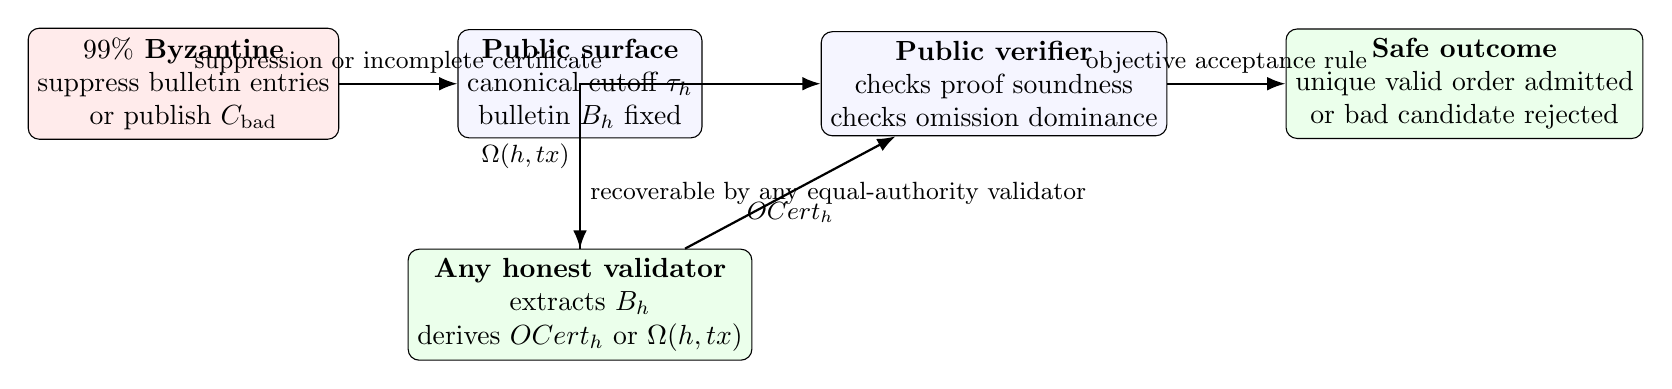
\begin{tikzpicture}[
  >=Latex,
  node distance=1.4cm and 1.5cm,
  stage/.style={draw, rounded corners, minimum width=3.05cm, minimum height=1.15cm, align=center, fill=blue!4},
  bad/.style={draw, rounded corners, minimum width=3.05cm, minimum height=1.15cm, align=center, fill=red!8},
  good/.style={draw, rounded corners, minimum width=3.05cm, minimum height=1.15cm, align=center, fill=green!8},
  note/.style={font=\small, align=center}
]
\node[bad] (attackers) {\textbf{\(99\%\) Byzantine}\\suppress bulletin entries\\or publish \(C_{\mathrm{bad}}\)};
\node[stage, right=of attackers] (bulletin) {\textbf{Public surface}\\canonical cutoff \(\tau_h\)\\bulletin \(B_h\) fixed};
\node[good, below=of bulletin] (recoverer) {\textbf{Any honest validator}\\extracts \(B_h\)\\derives \(OCert_h\) or \(\Omega(h, tx)\)};
\node[stage, right=of bulletin] (verifier) {\textbf{Public verifier}\\checks proof soundness\\checks omission dominance};
\node[good, right=of verifier] (outcome) {\textbf{Safe outcome}\\unique valid order admitted\\or bad candidate rejected};

\draw[->, thick] (attackers) -- node[above, note] {suppression or incomplete certificate} (bulletin);
\draw[->, thick] (bulletin) -- node[right, note] {recoverable by any equal-authority validator} (recoverer);
\draw[->, thick] (recoverer) -- node[below, note] {\(OCert_h\)} (verifier);
\draw[->, thick] (recoverer) |- node[pos=0.28, left, note] {\(\Omega(h, tx)\)} (verifier);
\draw[->, thick] (verifier) -- node[above, note] {objective acceptance rule} (outcome);
\end{tikzpicture}
\caption{Omission-dominance attack and deterministic extraction. Even if a
suppressing supermajority tries to hide admissible bulletin entries or promote
an incomplete candidate certificate, any honest validator that reconstructs the
same public surface derives the same valid \(OCert_h\) or publishes a valid
omission proof \(\Omega(h, tx)\) that kills the bad candidate.}
\label{fig:omission-dominance-recovery}
\end{figure}

The strongest shorthand is:
\[
99\% \text{ of validators may behave arbitrarily,}
\]
\[
\text{because the closed ordering boundary admits one deterministically}
\]
\[
\text{derivable close-or-abort outcome.}
\]

This is equal-authority because any validator may reveal the winning
certificate. It is \code{99\%}-fault tolerant because correctness does not
depend on a dense majority of positive votes. It is not classical
\code{99\% Byzantine agreement}.

With the accountable publication rules of
Section~\ref{sec:system-model}, invalid positive ordering attempts are not only
rejectable; they are also penalty-bearing and next-epoch removing.

\section{Asymptote: Sealed Finality and Irreversible Effects}

\code{Asymptote} is the two-tier settlement mode in the \AFT{} family. It
preserves fast \code{BaseFinal} chain progression while requiring stronger
evidence before irreversible effects are released.

\subsection{Finality tiers and collapse states}

The finality tiers are:

\begin{itemize}[leftmargin=1.5em]
\item \code{BaseFinal}: validator QC plus guardian certificate.
\item \code{SealedFinal}: \code{BaseFinal} plus sufficient sealing evidence.
\end{itemize}

The slot collapse states are:

\begin{itemize}[leftmargin=1.5em]
\item \code{Pending}
\item \code{BaseFinal}
\item \code{Sealing}
\item \code{Abort}
\item \code{SealedFinal}
\item \code{Escalated}
\item \code{Invalid}
\end{itemize}

All honest nodes must derive the same collapse state from the same admissible
evidence set.

\begin{figure}[t]
\centering
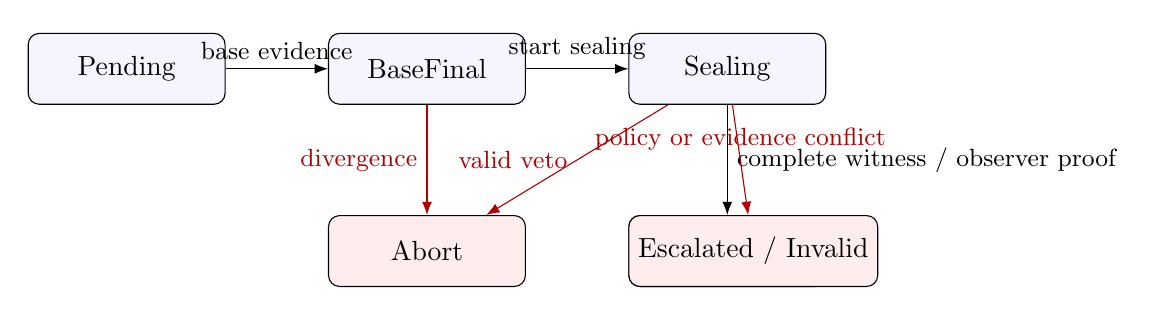
\begin{tikzpicture}[
  >=Latex,
  node distance=1.4cm and 1.3cm,
  state/.style={draw, rounded corners, minimum width=2.5cm, minimum height=0.9cm, align=center, fill=blue!4},
  bad/.style={draw, rounded corners, minimum width=2.5cm, minimum height=0.9cm, align=center, fill=red!7}
]
\node[state] (pending) {Pending};
\node[state, right=of pending] (base) {BaseFinal};
\node[state, right=of base] (sealing) {Sealing};
\node[state, below=of sealing] (sealed) {SealedFinal};
\node[bad, below=of base] (abort) {Abort};
\node[bad, right=of abort] (escalated) {Escalated / Invalid};

\draw[->] (pending) -- node[above, font=\small] {base evidence} (base);
\draw[->] (base) -- node[above, font=\small] {start sealing} (sealing);
\draw[->] (sealing) -- node[right, font=\small] {complete witness / observer proof} (sealed);
\draw[->, red!70!black] (sealing) -- node[left, font=\small] {valid veto} (abort);
\draw[->, red!70!black] (base) -- node[left, font=\small] {divergence} (abort);
\draw[->, red!70!black] (sealing) -- node[above, font=\small] {policy or evidence conflict} (escalated);
\end{tikzpicture}
\caption{The deterministic collapse surface for \code{Asymptote}.}
\end{figure}

\subsection{SealedFinalityProof}

The sealing plane gathers a proof object that binds:

\begin{itemize}[leftmargin=1.5em]
\item the epoch,
\item the achieved finality tier,
\item the collapse state,
\item the guardian manifest hash,
\item the guardian decision hash,
\item the guardian counter,
\item the guardian trace root,
\item the guardian measurement root,
\item the policy hash,
\item witness certificates, when the witness path is used,
\item observer transcripts, transcript commitment, observer challenges,
challenge commitment, and exactly one canonical observer outcome object when
the observer path is used,
\item divergence signals gathered during sealing.
\end{itemize}

This object is block-scoped and guardian-bound. A \code{SealedFinalityProof}
that is not bound to the slot's guardian evidence is invalid.

\subsection{Witness-backed sealing}

The witness path assigns one witness committee per required certification
stratum.

Witness assignment is deterministic over:

\begin{itemize}[leftmargin=1.5em]
\item the epoch seed,
\item the producer account id,
\item the slot \((height, view)\),
\item the reassignment depth,
\item the witness stratum id,
\item the witness manifest hash.
\end{itemize}

Sealed finality is reached on the witness path when:

\begin{itemize}[leftmargin=1.5em]
\item \code{BaseFinal} holds,
\item each required witness stratum contributes a valid assigned witness
certificate,
\item each witness certificate verifies against the registered witness manifest,
\item required checkpoints and append-only proofs are current enough under
policy.
\end{itemize}

Witness omission, stale registry participation, checkpoint inconsistency, or
conflicting witness certificates produce explicit evidence rather than silent
best-effort behavior.

\subsection{Equal-authority observer sealing}

The normative observer path is \code{CanonicalChallengeV1}. It treats sampled
validators as deterministic duty assignees whose outputs must become public,
recoverable protocol objects.

Observer assignment is deterministic over:

\begin{itemize}[leftmargin=1.5em]
\item the epoch seed,
\item the producer account id,
\item the slot \((height, view)\),
\item the observation round,
\item the observer account id.
\end{itemize}

The producer is excluded from its own observer pool. The runtime may also
filter assignments through a correlation budget over provider, region, host
class, and key-authority class.

Each assigned observer publishes one of two things:

\begin{itemize}[leftmargin=1.5em]
\item a guardian-backed \code{AsymptoteObserverTranscript}, or
\item an objective \code{AsymptoteObserverChallenge}.
\end{itemize}

A transcript binds the canonical slot surface:

\begin{itemize}[leftmargin=1.5em]
\item the epoch and assignment,
\item the candidate block hash,
\item the guardian manifest, decision hash, counter, trace hash, and
measurement root,
\item the guardian checkpoint root,
\item the observer verdict and veto kind,
\item the observer evidence hash.
\end{itemize}

The admissible challenge basis is public-evidence-only:

\begin{itemize}[leftmargin=1.5em]
\item \code{MissingTranscript},
\item \code{TranscriptMismatch},
\item \code{VetoTranscriptPresent},
\item \code{ConflictingTranscript},
\item \code{InvalidCanonicalClose}.
\end{itemize}

Each challenge carries its own public evidence object: an assignment, an
offending observation request, an offending transcript, or an offending
canonical close. The challenge \code{evidence\_hash} must bind exactly that
carried evidence.

The slot then carries three canonical bindings:

\begin{itemize}[leftmargin=1.5em]
\item a transcript commitment over the transcript surface,
\item a challenge commitment over the challenge surface,
\item exactly one canonical outcome object:
  \code{AsymptoteObserverCanonicalClose} or
  \code{AsymptoteObserverCanonicalAbort}.
\end{itemize}

The collapse rule is close-or-abort and challenge-dominant:

\begin{itemize}[leftmargin=1.5em]
\item \code{SealedFinal} if \code{BaseFinal} holds, the deterministic
assignment set is fully covered by valid canonical \code{Ok} transcripts, the
transcript and challenge commitments verify, the challenge surface is empty,
and the canonical close object is valid.
\item \code{Abort} if the transcript and challenge commitments verify, the
challenge surface is non-empty, and the canonical abort object is valid.
\item \code{Pending} otherwise.
\end{itemize}

This makes observer sealing structurally parallel to canonical ordering:
public evidence, canonical commitments, a unique positive object, a unique
negative object, and deterministic local close-or-abort derivation from the
same public surface.

\subsection{Divergence signals and escalation}

The sealing plane may also emit divergence signals, including:

\begin{itemize}[leftmargin=1.5em]
\item conflicting guardian certificates,
\item witness omission,
\item stale registry use,
\item stale checkpoints,
\item transparency-log consistency failure.
\end{itemize}

These signals support \code{Escalated} and \code{Invalid} outcomes and give
operators a fail-closed evidence trail.

\subsection{Sealed effects and replay-safe release}

Irreversible effects are gated by finality tier. The effect plane
distinguishes between:

\begin{itemize}[leftmargin=1.5em]
\item \code{BaseFinal} effects, which are allowed on the fast path when policy
permits,
\item \code{SealedFinal} effects, which require a valid
\code{SealedFinalityProof}.
\end{itemize}

For proof-enabled irreversible effects, \code{Asymptote} carries a
self-contained \code{SealObject} whose current instantiation includes:

\begin{itemize}[leftmargin=1.5em]
\item an \code{EffectIntent},
\item an \code{EffectPublicInputs} object, including
  \code{canonical\_collapse\_hash},
\item an \code{EffectProofEnvelope},
\item a replay-safe nullifier.
\end{itemize}

In the live runtime, \code{SealedFinal} secure-egress requests now carry both
the \code{SealedFinalityProof} and the slot's
\code{CanonicalCollapseObject}. The guardian-side seal builder and downstream
receipt verifier recompute the same \code{canonical\_collapse\_hash} from that
collapse object together with the proof-carried observer surface, so a
challenge-dominated or otherwise mismatched slot cannot authorize irreversible
release.

The release rule is
\[
\mathrm{Release}(e)
\iff
\mathrm{BaseFinal}(\mathrm{slot}(e))
\wedge
\mathrm{SealedFinal}(\mathrm{slot}(e))
\wedge
\mathrm{VerifySealObject}(e)
\wedge
\mathrm{CollapseHash}(e)=\mathrm{Hash}(\mathrm{Collapse}(\partial_h))
\wedge
\neg \mathrm{NullifierUsed}(e).
\]

This keeps the hot path sparse while making released consequences deterministic
and replay-safe.

\subsection{Deterministic observer theorem}

The deterministic \code{Asymptote} observer model now proves the following
kernel:

\begin{itemize}[leftmargin=1.5em]
\item base certificates are unique per slot,
\item canonical observer close objects are unique per slot,
\item canonical observer close and canonical observer abort cannot coexist for
the same slot,
\item a challenge-dominated slot cannot produce a valid sealed release.
\end{itemize}

\begin{theorem}[Deterministic Equal-Authority Observer Sealing]
Assume sound deterministic observer assignment, signature-sound guardian-backed
observer transcripts and challenges, canonical transcript and challenge
commitments, append-only registry and log publication once published, and
deterministic transcript/challenge derivation over the closed public observer
surface. Then arbitrary behavior by the rest of the validator set cannot create a
conflicting valid canonical observer close, cannot make canonical close and
canonical abort coexist for the same slot, and cannot authorize a valid sealed
irreversible effect release for a challenge-dominated slot.
\end{theorem}

This theorem is the observer-lane analogue of canonical ordering's public
certificate theorem: public evidence, canonical commitments, negative-authority
dominance, and deterministic local close-or-abort derivation from the same
public observer surface.

Under the accountable publication rules of
Section~\ref{sec:system-model}, the same observer challenges are also
penalty-bearing objective faults. Unsafe positive close attempts therefore
become not only rejectable, but accountable and epoch-removing.

\subsection{Legacy sampled comparison}

Before \code{CanonicalChallengeV1}, the observer lane was typically described
through a sampled affirmative bound. Let:

\begin{itemize}[leftmargin=1.5em]
\item \(h\) be the honest fraction of equal-authority validators,
\item \(A_s^j\) be the sampled observer committee for slot \(s\) and round
\(j\),
\item \(k_j = |A_s^j|\),
\item \(p_{\mathrm{beacon\_bias}}\) be the probability of sufficient beacon
bias,
\item \(p_{\mathrm{veto\_suppression}}\) be the probability that a valid veto
surface is fully suppressed.
\end{itemize}

Then the old affirmative sampled lane admitted the analytical bound
\[
P_{\mathrm{unsafe}}(s)
\le
p_{\mathrm{beacon\_bias}}
\cdot
p_{\mathrm{veto\_suppression}}
\cdot
\prod_j (1 - h)^{k_j}.
\]

For constant committee size \(k\) across \(r\) rounds:
\[
P_{\mathrm{unsafe}}(s)
\le
p_{\mathrm{beacon\_bias}}
\cdot
p_{\mathrm{veto\_suppression}}
\cdot
(1 - h)^{kr}.
\]

That formula remains a useful historical comparison, but it is no longer the
normative theorem for the observer lane. Under \code{CanonicalChallengeV1},
sampling determines duties, not safety. Safety comes from the canonical public
transcript surface, the canonical public challenge surface, and the
close-or-abort split that those surfaces induce.

The runtime publishes the canonical observer transcript, commitment, challenge,
challenge commitment, and close-or-abort objects as ordinary
\code{guardian\_registry} transactions after the sealed header is formed. The
same surface is carried inside the proof for immediate block verification.

\section{NestedGuardian: Witness-Augmented Research Mode}

\code{NestedGuardian} explores a layered threshold construction:

\begin{itemize}[leftmargin=1.5em]
\item validators run the \AFT{} deterministic message flow,
\item each proposal carries its guardian committee certificate,
\item external witness committees cross-check the slot,
\item chain state anchors witness assignments, witness manifests, and slashing
evidence.
\end{itemize}

The current runtime scope includes:

\begin{itemize}[leftmargin=1.5em]
\item deterministic witness assignment from the active witness set,
\item registered on-chain witness manifests,
\item witness certificates bound into guardianized slot certificates,
\item safety proofs for the witness-augmented kernel,
\item bounded model checking for reassignment, outage, and checkpoint
transitions.
\end{itemize}

The current proof status is intentionally narrow:

\begin{itemize}[leftmargin=1.5em]
\item safety is formalized,
\item operational transitions are model-checked in bounded scenarios,
\item composed liveness under repeated reassignment, outage, and rotation
remains open.
\end{itemize}

\code{NestedGuardian} should therefore be described as a witness-augmented
research path, not as a finished non-classical liveness theorem.

\section{Security and Assumption Surface}

The \AFT{} family depends on explicit assumptions. They are not optional prose.

\begin{center}
\small
\begin{tabularx}{\textwidth}{>{\raggedright\arraybackslash}p{0.17\textwidth} >{\raggedright\arraybackslash}p{0.42\textwidth} X}
\toprule
\textbf{Layer} & \textbf{Required assumptions} & \textbf{Failure consequence} \\
\midrule
Base finality & current manifests, current epoch state, majority thresholds, guardian non-equivocation, valid checkpoints, enough validators and guardians to reach quorum & conflicting base-finality evidence or loss of progress \\
Canonical ordering & objective publication, canonical cutoff, deterministic eligibility, append-only bulletin commitment, proof soundness, canonical bulletin-close extraction, cheap omission verification, accountable omission publication & loss of deterministic extraction, loss of accountability, or loss of the ordering theorem \\
Sealed finality & valid asymptote policy, current witness seed, valid witness or observer assignments, checkpoint freshness, valid log consistency proofs, deterministic transcript/challenge derivation, accountable challenge publication & incorrect sealed release, loss of accountability, or fail-closed stalling \\
Sealed effects & correct finality-tier policy, sound verifier metadata, nullifier uniqueness, intent/public-input binding & replay or unsafe irreversible effect release \\
NestedGuardian & sound witness assignment and registration, correct reassignment handling, witness committee non-equivocation & degraded safety or open liveness behavior \\
\bottomrule
\end{tabularx}
\end{center}

The family-level discipline is simple: if an assumption fails, \AFT{} should
degrade to stalling, aborting, or withholding release before it degrades to
unsafe irreversible behavior.

\section{Formal Results}

The repository's machine-checked surfaces align with the protocol family as
follows:

\begin{center}
\scriptsize
\begin{tabularx}{\textwidth}{>{\raggedright\arraybackslash}p{0.28\textwidth} X}
\toprule
\textbf{Formal module} & \textbf{Core proved results} \\
\midrule
\code{GuardianMajorityProof} & \code{QuorumCertificatesIntersect}, \code{InvariantImpliesSafety} \\
\code{GuardianMajority} & executable bounded checks for finalization witness soundness and slot safety \\
\code{CanonicalOrderingProof} & \shortstack[l]{\code{InvariantImpliesCertifiedUniqueness},\\\code{InvariantImpliesRecoverability},\\\code{InvariantImpliesOmissionDominates}} \\
\code{CanonicalOrdering} & executable bounded checks for publication, cutoff, certification, omission, and recoverability \\
\code{AsymptoteProof} & \shortstack[l]{\code{InvariantImpliesBaseSafety},\\\code{InvariantImpliesCanonicalCloseSafety},\\\code{InvariantImpliesCloseAbortExclusive},\\\code{InvariantImpliesAbortDominatesSealed}} \\
\code{Asymptote} & executable bounded checks for transcript publication, challenge publication, canonical close, and canonical abort \\
\code{NestedGuardianProof} & \shortstack[l]{witness-assignment soundness,\\witness-certificates-stay-assigned,\\\code{InvariantImpliesSafety}} \\
\code{NestedGuardian} & executable bounded checks for reassignment, outage, and checkpoint admissibility \\
\bottomrule
\end{tabularx}
\end{center}

These formal surfaces prove the deterministic safety kernels. They do not
prove classical unconditional \code{99\% Byzantine agreement}, nor do they
collapse environmental assumptions such as bulletin availability or challenge
publication and recoverability into pure algebraic theorems.

The accountable-adversary variant therefore composes these formal kernels with
runtime accountability rules rather than replacing them: replay-deduplicated
objective fault publication and optional policy-controlled membership updates
live in the implementation and policy layer above the proved
deterministic core.

\subsection{Representative omission-dominance trace}

In addition to invariant checking, the repository now carries an executable TLC
witness module,
\code{formal/aft/canonical\_ordering/CanonicalOrderingOmissionTrace.tla},
paired with
\code{formal/aft/canonical\_ordering/CanonicalOrderingOmissionTrace.cfg}. The
module intentionally asks TLC to violate the state predicate
\code{NoOmissionDominanceWitness} so that the checker emits a concrete public
evidence trace. The executed trace is:

\begin{enumerate}[leftmargin=1.5em]
\item \code{PublishStep}: \code{tx1} enters slot \(1\)'s bulletin surface.
\item \code{PublishStep}: \code{tx2} enters the same bulletin surface.
\item \code{CloseCutoffStep}: the canonical cutoff closes and the recoverable
set becomes \(\{tx1, tx2\}\).
\item \code{CandidateCertifyStep}: a candidate certificate for \(\{tx1\}\)
appears.
\item \code{ProveOmissionStep}: an omission proof for \(tx2\) against that
candidate certificate appears.
\end{enumerate}

The same formal package now also carries a bounded recursive-continuity model,
\code{formal/aft/canonical\_ordering/CanonicalCollapseRecursiveContinuity.tla},
paired with
\code{formal/aft/canonical\_ordering/CanonicalCollapseRecursiveContinuity.cfg}.
That model captures the reference \code{HashPcdV1} continuity carrier directly:
deterministic recursive proof steps, predecessor-proof hashing,
\code{CanonicalCollapseExtensionCertificate} carriage, and the rule that
non-genesis header admission depends on the anchored predecessor proof relation.
The runtime now also exposes a \code{SuccinctSp1V1} backend seam for those
same recursive public inputs, and that seam is now exercised by live consensus
verification and durable-state gating. The formal model still stops at the
reference carrier rather than mechanizing a cryptographic recursive
accumulator or ZK backend.

At the final state, the incomplete candidate certificate remains
\emph{unadmitted} while the omission proof is present. In the current executable
model this happens because the admitted object must already equal the canonical
set; the trace therefore does not replace the theorem. Its purpose is narrower
and useful: it gives a bounded, executed witness of the exact public-evidence
shape from which omission dominance follows. Readers can run the trace directly
and inspect the six-state witness without reconstructing the paper's argument by
hand.

\section{Implementation Correspondence}

This section is non-normative. It names the exact runtime symbols that carry
the protocol objects defined above.

\subsection{Core ordering symbols}

The core ordering data structures and free functions are public Rust symbols
re-exported through \code{ioi\_types::app}. They are the runtime carriers for
the abstract ordering objects and verifier rules defined above.

\begin{center}
\scriptsize
\begin{tabularx}{\textwidth}{>{\raggedright\arraybackslash}p{0.32\textwidth} X}
\toprule
\textbf{Abstract object} & \textbf{Current runtime symbols} \\
\midrule
Bulletin surface commitment & \code{BulletinCommitment}, \code{BulletinSurfaceEntry} \\
Canonical ordering proof families & \code{CanonicalOrderProofSystem}, with concrete variants \code{HashBindingV1} and \code{CommittedSurfaceV1} \\
Canonical public-input tuple & \code{CanonicalOrderPublicInputs} \\
Live succinct witness payload & \code{CommittedSurfaceCanonicalOrderProof} \\
Omission evidence & \code{OmissionProof} \\
Order certificate & \code{CanonicalOrderCertificate} \\
Canonical ordering function & \code{canonical\_order\_tx\_hashes} \\
Public-input hashing & \shortstack[l]{\code{canonical\_order\_public\_inputs},\\\code{canonical\_order\_public\_inputs\_hash}} \\
Reference proof construction & \shortstack[l]{\code{build\_reference\_canonical\_order}\\\code{\_proof\_bytes}} \\
Live certificate construction & \shortstack[l]{\code{build\_committed\_surface\_canonical}\\\code{\_order\_certificate}} \\
Certificate verification & \code{verify\_canonical\_order\_certificate} \\
\bottomrule
\end{tabularx}
\end{center}

\subsection{Guardian and sealing symbols}

The guardian, witness, observer, and sealed-effect objects are likewise public
Rust symbols re-exported through \code{ioi\_types::app}. They encode the exact
evidence surface checked by validators and downstream gateways.

\begin{center}
\small
\begin{tabularx}{\textwidth}{>{\raggedright\arraybackslash}p{0.32\textwidth} X}
\toprule
\textbf{Abstract object} & \textbf{Current runtime symbols} \\
\midrule
Guardian slot certificate & \code{GuardianQuorumCertificate} \\
Witness certificate & \code{GuardianWitnessCertificate} \\
Equal-authority observer assignment & \code{AsymptoteObserverAssignment} \\
Correlation budget & \code{AsymptoteObserverCorrelationBudget} \\
Observer observation request & \code{AsymptoteObserverObservationRequest} \\
Observer transcript & \code{AsymptoteObserverTranscript} \\
Observer transcript commitment & \code{AsymptoteObserverTranscriptCommitment} \\
Observer challenge & \code{AsymptoteObserverChallenge}, with kinds \code{MissingTranscript}, \code{TranscriptMismatch}, \code{VetoTranscriptPresent}, \code{ConflictingTranscript}, and \code{InvalidCanonicalClose} \\
Observer challenge commitment & \code{AsymptoteObserverChallengeCommitment} \\
Canonical observer close & \code{AsymptoteObserverCanonicalClose} \\
Canonical observer abort & \code{AsymptoteObserverCanonicalAbort} \\
Finality tier & \code{FinalityTier}, with variants \code{BaseFinal} and \code{SealedFinal} \\
Collapse state & \code{CollapseState}, with variants \code{Pending}, \code{BaseFinal}, \code{Sealing}, \code{Abort}, \code{SealedFinal}, \code{Escalated}, and \code{Invalid} \\
Sealing policy & \code{AsymptotePolicy} \\
Observer statement & \code{AsymptoteObserverStatement} \\
Observer certificate & \code{AsymptoteObserverCertificate} \\
Divergence signal & \code{DivergenceSignal}, \code{DivergenceSignalKind} \\
Sealed finality proof & \code{SealedFinalityProof} \\
Observer binding for sealed effects & \code{sealed\_finality\_proof\_observer\_binding} \\
Proof-carrying effect object & \code{SealObject} \\
\bottomrule
\end{tabularx}
\end{center}

\subsection{Verifier, orchestration, and persistence symbols}

Verification and orchestration entry points are split across four public
namespaces: \code{ioi\_types::app},
\code{ioi\_crypto::sign::guardian\_committee},
\code{ioi\_services::guardian\_registry}, and the
\code{GuardianMajorityEngine} runtime. Engine-local checks are named here by
their exact method identifiers.

\begin{center}
\scriptsize
\begin{tabularx}{\textwidth}{>{\raggedright\arraybackslash}p{0.37\textwidth} X}
\toprule
\textbf{Responsibility} & \textbf{Current runtime symbols} \\
\midrule
Guardian certificate verification & \code{verify\_quorum\_certificate} \\
Witness certificate verification & \code{verify\_witness\_certificate} \\
Deterministic observer assignment & \shortstack[l]{\code{derive\_asymptote\_observer\_assignments},\\\code{derive\_asymptote\_observer\_plan\_entries}} \\
Observer-side transcript / challenge derivation & \shortstack[l]{\code{GuardianContainer::observe\_asymptote\_request},\\\code{GuardianContainer::request\_remote\_asymptote}\\\code{\_observer\_observation},\\\code{GuardianContainer::sign\_consensus\_with\_guardian}} \\
Sealed finality verification in the engine & \shortstack[l]{\code{GuardianMajorityEngine::verify\_asymptote}\\\code{\_canonical\_observer\_sealed\_finality},\\\code{GuardianMajorityEngine::verify\_asymptote}\\\code{\_sealed\_finality}} \\
Canonical-order enrichment verification in the engine & \shortstack[l]{\code{GuardianMajorityEngine::verify}\\\code{\_canonical\_order\_enrichment}; published\\\code{CanonicalOrderAbort} dominates positive order\\certificates and inconsistent mixed parent state} \\
Block finalization attachment of order certificates & \shortstack[l]{\code{build\_committed\_surface\_canonical}\\\code{\_order\_certificate} during finalization} \\
Canonical observer proof publication & \shortstack[l]{\code{canonicalize\_observer\_sealed\_finality\_proof},\\\code{publish\_canonical\_observer\_artifacts}} \\
Sealed-effect construction and checking & \code{build\_http\_egress\_seal\_object}, \code{verify\_seal\_object} \\
Guardianized proposal verification in the engine & \shortstack[l]{\code{GuardianMajorityEngine::verify}\\\code{\_guardianized\_certificate}} \\
Base-engine safety and timing & \code{SafetyGadget}, \code{Pacemaker}, \code{TimeoutCertificate} \\
Bulletin and order-certificate state access & \shortstack[l]{\code{load\_bulletin\_commitment},\\\code{load\_canonical\_order\_certificate}} \\
Ordering close-or-abort derivation & \shortstack[l]{\code{derive\_canonical\_order\_execution\_object},\\\code{derive\_canonical\_order\_public\_obstruction}} \\
Ordering abort taxonomy & \shortstack[l]{\code{CanonicalOrderAbortReason::MissingOrderCertificate},\\\code{BulletinSurfaceReconstructionFailure},\\\code{BulletinSurfaceMismatch},\\\code{InvalidBulletinClose},\\\code{OmissionDominated},\\\code{CertificateHeightMismatch},\\\code{RandomnessMismatch},\\\code{OrderedTransactionsRootMismatch},\\\code{ResultingStateRootMismatch},\\\code{InvalidPublicInputsHash},\\\code{InvalidBulletinAvailabilityCertificate},\\\code{InvalidProofBinding}} \\
Protocol-wide collapse derivation and verification & \shortstack[l]{\code{derive\_canonical\_collapse\_object},\\\code{GuardianMajorityEngine::verify\_published}\\\code{\_canonical\_collapse\_object}} \\
Proposal-surface recursive continuity & \shortstack[l]{\code{BlockHeader::previous\_canonical\_collapse\_commitment\_hash},\\\code{BlockHeader::canonical\_collapse\_extension\_certificate},\\\code{CanonicalCollapseExtensionCertificate},\\\code{CanonicalCollapseCommitment},\\\code{verify\_block\_header\_canonical\_collapse\_evidence},\\\code{ConsensusDecision::ProduceBlock}} \\
Bulletin, order, and collapse state access & \shortstack[l]{\code{load\_bulletin\_commitment},\\\code{load\_canonical\_order\_certificate},\\\code{load\_canonical\_order\_abort},\\\code{load\_canonical\_collapse\_object}} \\
On-chain publication verbs & \shortstack[l]{\code{publish\_aft\_canonical\_order\_artifact\_bundle@v1},\\\code{publish\_aft\_canonical\_order\_abort@v1},\\\code{publish\_aft\_canonical\_collapse\_object@v1},\\\code{report\_aft\_omission@v1},\\\code{publish\_asymptote\_observer\_transcript@v1},\\\code{publish\_asymptote\_observer\_transcript\_commitment@v1},\\\code{report\_asymptote\_observer\_challenge@v1},\\\code{publish\_asymptote\_observer\_challenge\_commitment@v1},\\\code{publish\_asymptote\_observer\_canonical\_close@v1},\\\code{publish\_asymptote\_observer\_canonical\_abort@v1}} \\
Accountable evidence replay protection and validator removal & \shortstack[l]{\code{evidence\_id},\\\code{GuardianRegistry::apply\_accountable\_fault\_report},\\\code{GuardianRegistry::apply\_accountable\_membership\_updates}} \\
Native benchmark target & \code{benchmark\_throughput} \\
\bottomrule
\end{tabularx}
\end{center}

These symbols are named here so that the paper maps directly onto the current
runtime without making the reader chase separate prose specifications. In the
current implementation, validator finalization now publishes a protocol-visible
\code{CanonicalCollapseObject} through
\code{publish\_aft\_canonical\_collapse\_object@v1} after local post-commit
header enrichment, \code{guardian\_registry} exposes
\code{load\_canonical\_collapse\_object}, and
\code{GuardianMajorityEngine::verify\_published\_canonical\_collapse\_object}
cross-checks any published copy against the proof-carried header surface when
it is available. The externally finalized AFT commit path persists the same
object keyed by slot height, rather than treating ordering and sealing
close-or-abort evidence as loose enrichments detached from state persistence.
In the current proposal-surface continuity slice, validator orchestration now
signs both \code{previous\_canonical\_collapse\_commitment\_hash} and a typed
\code{CanonicalCollapseExtensionCertificate} into each produced AFT block
header.
In the current clean-break runtime slice, \code{CanonicalCollapseObject}
itself carries \code{continuity\_accumulator\_hash} and
\code{continuity\_recursive\_proof}, so the certificate now carries the
predecessor commitment plus predecessor proof hash rather than an explicit
carried ancestor vector, full predecessor collapse object, or predecessor
recursive proof object.
\code{Asymptote} leaders stall rather than produce when that required
extension certificate is unavailable, proposal verification recursively
checks that the carried predecessor commitment hash matches the signed
predecessor link, checks that the predecessor commitment's resulting state root matches the
signed parent-state root, and rechecks those carried public inputs against the
anchored predecessor collapse object when one is available. QC promotion
therefore relies on a reference recursive proof-carrying continuity relation
rather than on a recomputed predecessor digest alone, and only treats continuity-linked
headers as progress-bearing.

\section{Benchmark Context}

The performance evidence in this paper has two sources:

\begin{itemize}[leftmargin=1.5em]
\item literature-reported baselines for \code{HotStuff}, \code{Narwhal/Tusk},
and \code{Bullshark},
\item the repository's native \code{benchmark\_throughput} target for matched
\code{GuardianMajority} and \code{Asymptote} scenarios.
\end{itemize}

The purpose of this section is architectural positioning, not false
equivalence across unmatched environments.

\subsection{Paper-reported baselines}

\begin{center}
\small
\begin{tabularx}{\textwidth}{>{\raggedright\arraybackslash}p{0.28\textwidth} >{\raggedleft\arraybackslash}p{0.16\textwidth} >{\raggedleft\arraybackslash}p{0.16\textwidth} X}
\toprule
\textbf{System} & \textbf{Reported throughput} & \textbf{Reported latency} & \textbf{Source type} \\
\midrule
HotStuff baseline & 1{,}800 tx/s & 1 s & Narwhal/Tusk comparison setting \\
Narwhal-HotStuff & 130{,}000 tx/s & under 2 s & Narwhal/Tusk paper \\
Narwhal-HotStuff with additional workers & up to 600{,}000 tx/s & n/a & Narwhal/Tusk paper \\
Tusk & 160{,}000 tx/s & about 3 s & Narwhal/Tusk paper \\
Bullshark & 125{,}000 tx/s & about 2 s & Bullshark paper \\
\bottomrule
\end{tabularx}
\end{center}

The baseline interpretation is:

\begin{itemize}[leftmargin=1.5em]
\item \code{HotStuff} demonstrates the leader-based partially synchronous
baseline,
\item \code{Narwhal-HotStuff} demonstrates the gain from separating
dissemination from ordering,
\item \code{Bullshark} demonstrates high-throughput DAG-oriented ordering,
\item \AFT{} adds a new separation: order revelation and effect release are no
longer identified with dense positive voting.
\end{itemize}

\subsection{Native repository measurements}

The corrected native measurements below were produced on March 16, 2026 after
fixing three benchmark-path issues:

\begin{itemize}[leftmargin=1.5em]
\item transaction gossip now retries on \code{InsufficientPeers},
\item genesis status starts from a shared configured wall-clock timestamp,
\item the orchestrator retries shared-memory attachment before falling back.
\end{itemize}

The table separates a burst-latency probe from a bulk-throughput probe.

\begin{center}
\scriptsize
\resizebox{\textwidth}{!}{%
\begin{tabular}{lrrrrrrrrrrrr}
\toprule
scenario & validators & attempted & accepted & committed & blocks & inj. tps & sust. tps & p50 & p95 & p99 & sealed p50 & sealed p95 \\
\midrule
guardian\_majority\_4v\_burst & 4 & 512 & 512 & 512 & 3 & 11214.96 & 36.43 & 487.49 & 11390.70 & 11398.07 & -- & -- \\
guardian\_majority\_4v\_bulk & 4 & 8192 & 8192 & 8192 & 2 & 13048.99 & 252.66 & 9276.35 & 32416.37 & 32419.21 & -- & -- \\
\bottomrule
\end{tabular}%
}
\end{center}

These measurements imply four things:

\begin{itemize}[leftmargin=1.5em]
\item the earlier single-digit TPS report was an artifact of benchmark-path
bugs,
\item ingress is not the immediate bottleneck,
\item the current repository is bottlenecked more by commit and state handling
than by raw publish rate,
\item the implementation remains far from the intended \code{8k--16k TPS}
target.
\end{itemize}

These numbers should therefore be read as corrected repository baselines, not
as optimized ceilings and not as apples-to-apples claims against the published
Narwhal/Bullshark environments.

\section{Related Work}

Geeq's Proof of Honesty (PoH) is important prior work in the ``99\%'' direction:
it argues for globally honest and canonical chain recovery in pure software
under assumptions including at least one honest node and an honest relay, and
it uses public evidence plus user-side verification to push beyond ordinary
dense-vote intuition \cite{geeq}. \AFT{} differs in a key respect: it is
relay-free and coordinator-free. Correctness does not depend on any designated
honest relay, broadcaster, or privileged recovery role. Instead, durable
ordering and sealed effects collapse through protocol-native public-evidence
objects whose negative forms are immediately decisive.

Narwhal/Tusk and Bullshark separate dissemination from ordering, but they still
ground ordering safety in dense positive certificates and quorum-intersection
arguments over the ordered object itself \cite{narwhal,bullshark}. HoneyBadgerBFT
and Dumbo move to asynchronous common-subset or MVBA-style agreement, but they
still rely on classical Byzantine-majority thresholds rather than a
public-state-continuity theorem over a canonical public surface
\cite{honeybadger,dumbo}. Chainlink CCIP and optimistic cross-chain mechanisms
add secondary monitoring layers, risk-management committees, or challenge
windows to detect and halt bad transfers, but the decisive recovery rule is
operational or economic rather than the immediate acceptance of a uniquely valid
proof-carrying canonical object recoverable by any equal-authority validator
\cite{ccip}. Accountable subgroup multisigs and finality gadgets add
equivocation evidence and slashing, yet still keep dense subgroup votes as the
positive safety object \cite{grandpa,accountable}. \AFT{} differs by making
ordering and sealed release relay-free public-evidence close-or-abort objects
with dominant negative proofs: honest validators that observe the same closed
public boundary derive the same decisive object, and publication is downstream
of that deterministic derivation rather than its source.

\section{Claims and Non-Claims}

\subsection{Claims}

This paper claims:

\begin{itemize}[leftmargin=1.5em]
\item a production guardian-backed base-finality model in which validator
quorums are composed with guardian committee admissibility,
\item proof-carrying canonical ordering with omission dominance, uniqueness,
and recoverability,
\item a public-state-continuity formulation in which closed slot boundaries
admit at most one positive public execution object and conflicting candidates
admit short objective obstruction witnesses,
\item \code{99\%} equal-authority ordering consensus under explicit
assumptions,
\item deterministic sealed-effect collapse with challenge dominance,
\item a relay-free, coordinator-free, pure-software public-state-continuity
theorem yielding deterministic \code{99\% Byzantine Tolerance} for durable
ordering and sealed-effect safety over the explicit bulletin / recoverability
substrate,
\item a witness-augmented research path for layered threshold constructions,
\item machine-checked deterministic safety kernels for the major protocol
surfaces.
\end{itemize}

\subsection{Non-claims}

This paper does \textbf{not} claim:

\begin{itemize}[leftmargin=1.5em]
\item unconditional classical \code{99\% Byzantine agreement} in the dense-vote
hidden-behavior model,
\item that public state continuity arises for free inside the classical DLS /
PBFT partially synchronous message-passing model,
\item freedom from bulletin-publication, availability, or proof-soundness
assumptions,
\item a full asynchronous liveness theorem under arbitrary registry, log,
witness, and outage schedules,
\item an apples-to-apples measured throughput superiority over
\code{HotStuff}, \code{Narwhal}, \code{Tusk}, or \code{Bullshark} from the
current repository alone.
\end{itemize}

\subsection{Public-state-continuity theorem}
\label{sec:accountable-ba}

The live runtime now supports a stronger theorem than the older accountable
revelation phrasing, provided the substrate model is stated honestly.

\begin{theorem}[Relay-Free Deterministic 99\% Byzantine Tolerance]
Assume the system model of Section~\ref{sec:system-model}, guardian
non-equivocation, proof soundness, canonical bulletin-close extraction for
ordering, deterministic transcript/challenge derivation for sealing, durable
state advancement only through canonical collapse, and irreversible-effect
release only through collapse-bound sealed proofs. Then up to \(99\%\) of
validators may behave arbitrarily without creating a conflicting valid durable
canonical-order outcome or a conflicting valid sealed-effect release outcome.
Honest validators that observe the same closed public boundary derive the same
close-or-abort result; publication, penalties, and validator-set updates only
accelerate convergence and future hygiene. This is Byzantine tolerance over the
public-state-continuity substrate, not classical dense-vote Byzantine
agreement.
\end{theorem}

The theorem is stronger than the older accountable revelation summary because
invalid positive objects are not merely rejectable or penalty-bearing. They are
already dominated by deterministic negative objects and collapse-gated durable
state before any penalty logic runs.

\begin{theorem}[Separation Statement]
\AFT{}'s \code{99\% Byzantine Tolerance} claim does not arise for free from the
classical DLS / PBFT partially synchronous authenticated message-passing model
alone. It depends essentially on the stronger public-state-continuity
substrate: canonical bulletin-close extraction, dominant negative objects, and
collapse-gated durability. Removing that substrate collapses the theorem back
toward the classical dense-vote frontier.
\end{theorem}

This should be read in deliberate contrast to classical partially synchronous
Byzantine agreement. In the classical dense-vote model, worst-case progress
requires \(> 2/3\) honest participation and quorum intersection is the main
safety mechanism. In \AFT{}'s PSC model, safety instead comes from uniquely
valid public-evidence objects plus dominant negative proofs, without trusted
relays, privileged coordinators, TEEs, or dense positive quorum intersection.
Publication and accountability serve as reinforcement rather than the source of
correctness. Liveness then follows from the availability of the PSC substrate
and eventual publication of the protocol-defined artifacts, not from assuming a
dense honest supermajority on the hot path.

The correct one-line summary is:

\begin{quote}
\AFT{} is a proof-carrying, guardian-backed, omission-dominant consensus and
settlement family in which base finality, canonical ordering, and
irreversible-effect release are separated and then recomposed through shared
evidence.
\end{quote}

\begin{thebibliography}{99}

\bibitem{hotstuff}
Maofan Yin, Dahlia Malkhi, Michael K.~Reiter, Guy Golan-Gueta, and Ittai
Abraham.
\newblock \emph{HotStuff: BFT Consensus in the Lens of Blockchain}.
\newblock arXiv:1803.05069.
\newblock \url{https://arxiv.org/abs/1803.05069}

\bibitem{narwhal}
George Danezis, Lefteris Kokoris-Kogias, Alberto Sonnino, and Alexander
Spiegelman.
\newblock \emph{Narwhal and Tusk: A DAG-based Mempool and Efficient BFT
Consensus}.
\newblock arXiv:2105.11827.
\newblock \url{https://arxiv.org/abs/2105.11827}

\bibitem{bullshark}
Ittai Abraham, Dahlia Malkhi, Kartik Nayak, Ling Ren, and Alexander Spiegelman.
\newblock \emph{Bullshark: DAG BFT Protocols Made Practical}.
\newblock arXiv:2201.05677.
\newblock \url{https://arxiv.org/abs/2201.05677}

\bibitem{honeybadger}
Andrew Miller, Yu Xia, Kyle Croman, Elaine Shi, and Dawn Song.
\newblock \emph{The Honey Badger of BFT Protocols}.
\newblock Proceedings of the 2016 ACM SIGSAC Conference on Computer and
Communications Security.
\newblock \url{https://eprint.iacr.org/2016/199.pdf}

\bibitem{dumbo}
Bingyong Guo, Zhenliang Lu, Qiang Tang, Jing Xu, and Zhenfeng Zhang.
\newblock \emph{Dumbo: Faster Asynchronous BFT Protocols}.
\newblock Proceedings of the 2020 ACM SIGSAC Conference on Computer and
Communications Security.
\newblock \url{https://dblp.org/rec/conf/ccs/GuoL0XZ20}

\bibitem{grandpa}
Alistair Stewart and Eleftherios Kokoris-Kogias.
\newblock \emph{GRANDPA: a Byzantine Finality Gadget}.
\newblock arXiv:2007.01560.
\newblock \url{https://arxiv.org/abs/2007.01560}

\bibitem{accountable}
Jelena Dosenovic, Roger Wattenhofer, and others.
\newblock \emph{Accountable Safety Implies Finality}.
\newblock arXiv:2308.16902.
\newblock \url{https://arxiv.org/abs/2308.16902}

\bibitem{ccip}
Chainlink Labs.
\newblock \emph{Chainlink CCIP's Defense-In-Depth Security and the Risk
Management Network}.
\newblock Chainlink blog, 2023.
\newblock \url{https://blog.chain.link/ccip-risk-management-network/}

\bibitem{geeq}
John P.~Conley.
\newblock \emph{Proof of Honesty: Coalition-Proof Blockchain Validation without
Proof of Work or Stake}.
\newblock Geeq technical paper, version 2.0, 2019.
\newblock \url{https://geeq.io/wp-content/uploads/GEEQ-OFFICIAL-TECHNICAL-PAPER.pdf}

\bibitem{halo}
Sean Bowe, Jack Grigg, and Daira Hopwood.
\newblock \emph{Halo: Recursive Proof Composition without a Trusted Setup}.
\newblock IACR ePrint 2019/1021.
\newblock \url{https://eprint.iacr.org/2019/1021}

\bibitem{pcd}
Benedikt B{\"u}nz, Alessandro Chiesa, Pratyush Mishra, and Nicholas Spooner.
\newblock \emph{Proof-Carrying Data from Accumulation Schemes}.
\newblock IACR ePrint 2020/499.
\newblock \url{https://eprint.iacr.org/2020/499}

\end{thebibliography}

\end{document}
